\documentclass[11pt,a4paper]{article}

% ===============================
% Foundations: Fonts, Encoding, Space
% ===============================
\usepackage{iftex}
\usepackage[T1]{fontenc}
\usepackage[utf8]{inputenc}
\usepackage{lmodern}        % modern Latin Modern (fixes small-caps warnings via ssub below)
\usepackage{microtype}
\usepackage{geometry}
\geometry{margin=1in}
\usepackage{setspace}
\onehalfspacing

% Provide a fallback for bold+smallcaps to avoid T1/lmr/bx/sc warning
\makeatletter
\AtBeginDocument{%
  % Map bold+smallcaps (bx/sc) to medium+smallcaps (m/sc) for the *current* roman family.
  \DeclareFontShape{T1}{\rmdefault}{bx}{sc}{<->ssub*\rmdefault/m/sc}{}%
}
\makeatother

% ===============================
% Language & Basics
% ===============================
\usepackage[english]{babel}
\usepackage{csquotes}
\usepackage{booktabs, array, multirow}
\usepackage{enumitem}
\setlist{nosep}

% ===============================
% Math
% ===============================
\usepackage{mathtools, amsmath, amssymb, amsthm, bm}
\numberwithin{equation}{section}

% Theorem styles
\theoremstyle{plain}
\newtheorem{theorem}{Theorem}[section]
\newtheorem{lemma}[theorem]{Lemma}
\theoremstyle{definition}
\newtheorem{definition}[theorem]{Definition}
\theoremstyle{remark}
\newtheorem{remark}[theorem]{Remark}

% Notation
\DeclareMathOperator*{\argmin}{arg\,min}
\DeclareMathOperator{\supp}{supp}
\newcommand{\bbR}{\mathbb{R}}
\newcommand{\bbP}{\mathbb{P}}
\newcommand{\calX}{\mathcal{X}}
\newcommand{\calQ}{\mathcal{Q}}    % set of receipt chains (abstract)
\newcommand{\join}{\sqcup}         % lattice join

% ===============================
% Graphics & TikZ
% ===============================
\usepackage{graphicx}
\usepackage[dvipsnames]{xcolor}
\usepackage{tikz}
\usetikzlibrary{arrows.meta,calc,positioning,fit,patterns,shapes.symbols}

\tikzset{
  block/.style     = {draw, rounded corners=3pt, align=center, inner sep=4pt, fill=gray!6},
  smallblock/.style= {block, font=\footnotesize, inner sep=2pt},
  line/.style      = {->, very thick, >={Stealth[length=2.5mm]}},
  dashedline/.style= {line, dashed},
}

% ===============================
% Unicode Hygiene (safe pasting)
% ===============================
\usepackage{newunicodechar}
\newunicodechar{–}{--}
\newunicodechar{—}{---}
\newunicodechar{…}{\ldots}
\newunicodechar{→}{\textrightarrow}
\newunicodechar{←}{\textrightarrow}
\newunicodechar{↔}{\ensuremath{\leftrightarrow}}
\newunicodechar{≤}{\ensuremath{\le}}
\newunicodechar{≥}{\ensuremath{\ge}}
\newunicodechar{≠}{\ensuremath{\ne}}
\newunicodechar{•}{\textbullet}

% ===============================
% Hyperref (safe metadata; no math in PDF strings)
% ===============================
\usepackage[unicode,colorlinks=true,linkcolor=MidnightBlue,citecolor=ForestGreen,urlcolor=RoyalBlue]{hyperref}
\hypersetup{
  pdftitle    ={Normalized, Verifiable Computation: A Safety-First Proposal},
  pdfauthor   ={},
  pdfsubject  ={},
  pdfkeywords ={}
}
\pdfstringdefDisableCommands{%
  \def\to{to}%
  \def\bm#1{#1}%
  \def\ensuremath#1{#1}%
}

% Helper for headings with math:
\newcommand{\mtitle}[2]{\texorpdfstring{#1}{#2}}

% ===============================
% Title
% ===============================
\title{Normalized, Verifiable Computation: A Safety-First Proposal}
\author{}
\date{\today}

% ===============================
% Document
% ===============================
\begin{document}
\maketitle

\begin{abstract}
We present a neutral, safety-first proposal for verifiable computation that treats trust as auditable evidence rather than assumption. The framework combines: (i) norm specifications with quantitative semantics suitable for automated checks; (ii) a compositional evidence layer where receipts chain deterministically and aggregate via join; and (iii) deterministic execution with selective disclosure, enabling independent verification while minimizing exposure. We include a practical batching/ledger pattern, lightweight runtime certificates, a cache-and-revocation path for heavier proofs, and a monotone governance gate that prevents safety regression.
\end{abstract}

\section{Overview}
This manuscript outlines a minimal but complete stack for high-assurance computation:
\begin{enumerate}[label=\textbf{O\arabic*}.]
  \item \textbf{Norms} with quantitative semantics (e.g., temporal guards with robustness) and a bounded SMT gate.
  \item \textbf{Evidence} as signed, canonical receipts that chain via digests and admit a join operation for parallel provenance.
  \item \textbf{Determinism} via frozen environments and canonical encodings; reproducibility attested by a proof-surface root.
  \item \textbf{Privacy} through commit–reveal selective disclosure at field granularity.
  \item \textbf{Governance} with monotone safety (must-fail sets cannot shrink) and auditable policy-as-code.
\end{enumerate}
The aim is a normalized baseline that others can extend, analyze, and critique.

\section{Norms with Quantitative Semantics and Bounded Checking}
Let time be discrete $t\in\mathbb{N}$. System metrics are signals $x:\mathbb{N}\to\bbR^d$. A guard $\varphi$ has a robustness $\rho(\varphi,x,t)\in\bbR$; $\rho>0$ implies satisfaction, $\rho<0$ violation. Examples include:
\begin{itemize}
  \item \emph{Safety band}:\; $\rho = \min_i \{\,u_i - x_i(t),\; x_i(t) - \ell_i\,\}$.
  \item \emph{Dwell/latency}:\; time-bounded ``globally'' and ``eventually'' constraints with quantitative semantics.
\end{itemize}
A \emph{Norms Bundle} is a finite set of such guards with parameters (thresholds, windows) and a set $M$ of \emph{must-fail} checks. A bounded-horizon SMT translation serves as a pre-merge gate.

\begin{lemma}[Monotone upgrade check]
If $M_{\mathrm{old}}\subseteq M_{\mathrm{new}}$ and all updated guards are unchanged or tightened (nondecreasing $\rho$ lower bounds under the same monitoring discretization), then the feasible region of safe behavior does not expand, i.e., no regression in safety posture occurs under the gate.
\end{lemma}

\begin{proof}[Sketch]
Must-fail inclusion blocks removal of failure classes. Tightening guards reduces or preserves feasible sets under bounded unfolding; CI rejects any weakening. \end{proof}

\section{Compositional Evidence: Chains and Join}
Receipts are signed headers over canonical encodings (JSON RFC 8785 or CBOR RFC 8949); transcripts, inputs, and outputs are referenced by digest. Let $\calQ$ be the set of finite, acyclic \emph{chains} plus a bottom $\bot$ (invalid). We define:
\begin{itemize}
  \item \textbf{Sequential composition} $c_2 * c_1 = c_2$ if $c_2.\texttt{prev\_digest} = H(c_1)$; else $\bot$.
  \item \textbf{Join} $\join$ as a Merkle-supremum over a set of chains (commitment to their union via a root).
  \item \textbf{Absorber} $\bot$ is fail-closed under both $*$ and $\join$.
\end{itemize}
This yields a practical algebra: temporal evolution via $*$; concurrent aggregation via $\join$. Domain-separated hashing and genesis receipts avoid cross-domain collisions.

\begin{lemma}[Distributivity (sketch at header level)]
For a chain $c$ and a family $\{q_i\}$,
\[
  c * \big(\join_i q_i\big) \;\equiv\; \join_i (c * q_i),
\]
since linking by previous digest composes with the union committed by the Merkle root, and canonicalization makes the commitment order-insensitive.
\end{lemma}

\section{Runtime Certificates: Lightweight First, Heavy Later}
\textbf{Level-1 (always-on):}
\begin{itemize}
  \item \emph{KKT receipts}: residuals and duality-gap bounds for convex subproblems with problem-class tag.
  \item \emph{Conservation receipts}: declared budget spend vs.\ observed potential change within tolerance.
\end{itemize}
\textbf{Level-2 (cached):} heavier proofs (e.g., passivity or ISS margins) are accepted from an audited cache keyed by component digests, with revocation checks. All verdicts are recorded as receipts.

\section{Determinism and Reproducibility}
Determinism is enforced by:
\begin{itemize}
  \item \emph{Envlock}: frozen toolchain and OS image (referenced by digest).
  \item \emph{Canonical encodings}: RFC 8785 JSON or deterministic CBOR.
  \item \emph{Seeds}: explicit PRNG seeds for stochastic steps used only for robustness probes.
\end{itemize}
Reproducibility is summarized by a \emph{proof surface}: a Merkle root over canonical receipt headers across batches. Cross-platform replay requires root equality; divergence triggers diagnostics.

\section{Batching, Proof Surfaces, and Archival}
A deterministic BLT-style pipeline processes data in batches. Each batch emits a transcript and a receipt with \texttt{prev\_digest} linking. Periodic epoch summaries commit to historical roots, enabling migration of old receipts to cold storage while preserving verifiability.

\section{Selective Disclosure and Privacy}
Each receipt header commits to a payload Merkle root. Verification tasks reveal only necessary fields with Merkle paths. This commit–reveal method minimizes exposure while preserving end-to-end auditability. Policies can require inequality proofs without raw values when thresholds suffice.

\section{Trust Metric (Transparent Hooks)}
Trust is computed from auditable components (e.g., certificate pass rates, robustness margins, drift indicators). Where needed, calibration (e.g., isotonic regression) is stored as a signed artifact and applied at presentation. Score intervals or bands are preferred when inputs are stale.

\section{Illustrative Figure (Deterministic Pipeline)}
\begin{figure}[t]
  \centering
  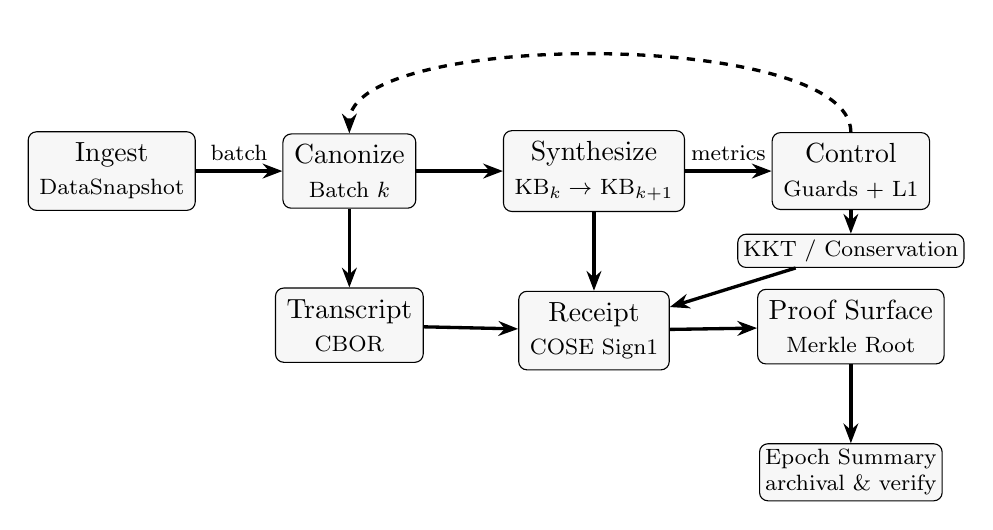
\begin{tikzpicture}[node distance=14mm and 11mm]
    % Execution path
    \node[block] (ingest) {Ingest\\ \footnotesize DataSnapshot};
    \node[block, right=of ingest] (canon) {Canonize\\ \footnotesize Batch $k$};
    \node[block, right=of canon] (synth) {Synthesize\\ \footnotesize KB$_k \to$ KB$_{k+1}$};
    \node[block, right=of synth] (control) {Control\\ \footnotesize Guards + L1};

    % Evidence artifacts
    \node[block, below=10mm of canon] (transcript) {Transcript\\ \footnotesize CBOR};
    \node[block, below=10mm of synth] (receipt) {Receipt\\ \footnotesize COSE Sign1};
    \node[block, below=10mm of control] (proof) {Proof Surface\\ \footnotesize Merkle Root};

    % Edges: execution flow
    \draw[line] (ingest) -- (canon) node[midway, above, sloped, font=\footnotesize] {batch};
    \draw[line] (canon) -- (synth);
    \draw[line] (synth) -- (control) node[midway, above, font=\footnotesize] {metrics};

    % Edges: evidence layer
    \draw[line] (canon) -- (transcript);
    \draw[line] (synth) -- (receipt);
    \draw[line] (transcript) -- (receipt);
    \draw[line] (receipt) -- (proof);

    % Certification spur (L1)
    \node[smallblock, below=3mm and of control] (kkt) {KKT / Conservation};
    \draw[line] (control) -- (kkt);
    \draw[line] (kkt) -- (receipt);

    % Closed-loop governance hint
    \draw[dashedline] (control) .. controls +(0,1.8) and +(0,1.8) .. (canon);

    % Epoch summary / archival
    \node[smallblock, below=10mm of proof] (summary) {Epoch Summary\\ \footnotesize archival \& verify};
    \draw[line] (proof) -- (summary);
  \end{tikzpicture}
  \caption{Deterministic pipeline with transcripts, receipts, and a proof-surface root. The figure is robust to Overleaf: all coordinates use \texttt{calc} node math and never reference undefined shapes.}
  \label{fig:pipeline}
\end{figure}

\section{Threat Model (Brief) and Mitigations}
\textbf{Tamper}: hash-chained receipts, proof-surface roots, non-malleable signatures. \\
\textbf{Non-determinism}: envlock, canonical encodings, seeded probes. \\
\textbf{Overload}: deterministic batching, rate limits, epoch summaries. \\
\textbf{Regression}: monotone norms enforced in CI. \\
\textbf{Privacy}: field-level commit–reveal proofs.

\section{Evaluation Plan (Abbreviated)}
\textbf{Replay}: cross-platform equality of proof-surface roots. \\
\textbf{Tamper injections}: single-byte mutations must break verification. \\
\textbf{Certification efficacy}: L1 true/false positive characterization. \\
\textbf{Scaling}: throughput/latency for batch receipts and root construction. \\
\textbf{Calibration}: trust-score reliability against independent audits.

\section{Conclusion}
We propose a normalized baseline for verifiable computation, emphasizing precise norms, compositional evidence, deterministic execution, and selective disclosure. A monotone governance gate and transparent trust hooks aim to keep assurance improving with use while minimizing disclosure.

% References placeholder (optional)
% \bibliographystyle{abbrv}
% \bibliography{refs}

\end{document}
